\documentclass[12pt, titlepage]{article}

\usepackage{fullpage}
\usepackage[round]{natbib}
\usepackage{multirow}
\usepackage{booktabs}
\usepackage{tabularx}
\usepackage{graphicx}
\usepackage{float}
\usepackage{hyperref}
\hypersetup{
    colorlinks,
    citecolor=blue,
    filecolor=black,
    linkcolor=red,
    urlcolor=blue
}

%% Comments

\usepackage{color}

\newif\ifcomments\commentstrue %displays comments
%\newif\ifcomments\commentsfalse %so that comments do not display

\ifcomments
\newcommand{\authornote}[3]{\textcolor{#1}{[#3 ---#2]}}
\newcommand{\todo}[1]{\textcolor{red}{[TODO: #1]}}
\else
\newcommand{\authornote}[3]{}
\newcommand{\todo}[1]{}
\fi

\newcommand{\wss}[1]{\authornote{blue}{SS}{#1}} 
\newcommand{\plt}[1]{\authornote{magenta}{TPLT}{#1}} %For explanation of the template
\newcommand{\an}[1]{\authornote{cyan}{Author}{#1}}

%% Common Parts

\newcommand{\progname}{ProgName} % PUT YOUR PROGRAM NAME HERE
\newcommand{\authname}{Team \#, Team Name
\\ Student 1 name
\\ Student 2 name
\\ Student 3 name
\\ Student 4 name} % AUTHOR NAMES                  

\usepackage{hyperref}
    \hypersetup{colorlinks=true, linkcolor=blue, citecolor=blue, filecolor=blue,
                urlcolor=blue, unicode=false}
    \urlstyle{same}
                                


\newcounter{acnum}
\newcommand{\actheacnum}{AC\theacnum}
\newcommand{\acref}[1]{AC\ref{#1}}

\newcounter{ucnum}
\newcommand{\uctheucnum}{UC\theucnum}
\newcommand{\uref}[1]{UC\ref{#1}}

\newcounter{mnum}
\newcommand{\mthemnum}{M\themnum}
\newcommand{\mref}[1]{M\ref{#1}}

\begin{document}

\title{Module Guide for Pot-Pulator} 
\author{Team 24  \\ Gillian Ford\\ Juan Moncada \\ Aaron Billones  \\ Steven Ramundi }
\date{\today}

\maketitle

\pagenumbering{roman}

\section{Revision History}

\begin{tabularx}{\textwidth}{p{3cm}p{2cm}X}
\toprule {\bf Date} & {\bf Version} & {\bf Notes}\\
\midrule
2023-01-07 & 1.0 & initial release\\
\\
\bottomrule
\end{tabularx}

\newpage

\section{Reference Material}

This section records information for easy reference.

\subsection{Abbreviations and Acronyms}

\renewcommand{\arraystretch}{1.2}
\begin{tabular}{l l} 
  \toprule		
  \textbf{symbol} & \textbf{description}\\
  \midrule 
  AC & Anticipated Change\\
  DAG & Directed Acyclic Graph \\
  M & Module \\
  MG & Module Guide \\
  OS & Operating System \\
  R & Requirement\\
  SC & Scientific Computing \\
  SRS & Software Requirements Specification\\
  \progname & Explanation of program name\\
  UC & Unlikely Change \\
  \bottomrule
\end{tabular}\\

\newpage

\tableofcontents

\listoftables

\listoffigures

\newpage

\pagenumbering{arabic}

\section{Introduction}

Decomposing a system into modules is a commonly accepted approach to developing
software.  A module is a work assignment for a programmer or programming
team~\citep{ParnasEtAl1984}.  We advocate a decomposition
based on the principle of information hiding~\citep{Parnas1972a}.  This
principle supports design for change, because the ``secrets'' that each module
hides represent likely future changes.  Design for change is valuable in SC,
where modifications are frequent, especially during initial development as the
solution space is explored.  

Our design follows the rules layed out by \citet{ParnasEtAl1984}, as follows:
\begin{itemize}
\item System details that are likely to change independently should be the
  secrets of separate modules.
\item Each data structure is implemented in only one module.
\item Any other program that requires information stored in a module's data
  structures must obtain it by calling access programs belonging to that module.
\end{itemize}

After completing the first stage of the design, the Software Requirements
Specification (SRS), the Module Guide (MG) is developed~\citep{ParnasEtAl1984}. The MG
specifies the modular structure of the system and is intended to allow both
designers and maintainers to easily identify the parts of the software.  The
potential readers of this document are as follows:

\begin{itemize}
\item New project members: This document can be a guide for a new project member
  to easily understand the overall structure and quickly find the
  relevant modules they are searching for.
\item Maintainers: The hierarchical structure of the module guide improves the
  maintainers' understanding when they need to make changes to the system. It is
  important for a maintainer to update the relevant sections of the document
  after changes have been made.
\item Designers: Once the module guide has been written, it can be used to
  check for consistency, feasibility, and flexibility. Designers can verify the
  system in various ways, such as consistency among modules, feasibility of the
  decomposition, and flexibility of the design.
\end{itemize}

The rest of the document is organized as follows. Section
\ref{SecChange} lists the anticipated and unlikely changes of the software
requirements. Section \ref{SecMH} summarizes the module decomposition that
was constructed according to the likely changes. Section \ref{SecConnection}
specifies the connections between the software requirements and the
modules. Section \ref{SecMD} gives a detailed description of the
modules. Section \ref{SecTM} includes two traceability matrices. One checks
the completeness of the design against the requirements provided in the SRS. The
other shows the relation between anticipated changes and the modules. Section
\ref{SecUse} describes the use relation between modules.

\section{Anticipated and Unlikely Changes} \label{SecChange}

This section lists possible changes to the system. According to the likeliness
of the change, the possible changes are classified into two
categories. Anticipated changes are listed in Section \ref{SecAchange}, and
unlikely changes are listed in Section \ref{SecUchange}.

\subsection{Anticipated Changes} \label{SecAchange}

Anticipated changes are the source of the information that is to be hidden
inside the modules. Ideally, changing one of the anticipated changes will only
require changing the one module that hides the associated decision. The approach
adapted here is called design for
change.

\begin{description}
\item[\refstepcounter{acnum} \actheacnum \label{acphy}:] The physical input
devices that the user will have available to them.
\item[\refstepcounter{acnum} \actheacnum \label{accal}:] Calulations for timing conveyor
stopage and movement.
\item[\refstepcounter{acnum} \actheacnum \label{acsen}:] Sensors used for verification and 
validation.(increased accurasy and lower latency)
\item[\refstepcounter{acnum} \actheacnum \label{accom}:] Communication protocol used to 
between the individual modules amd main board.

\end{description}

\subsection{Unlikely Changes} \label{SecUchange}

The module design should be as general as possible. However, a general system is
more complex. Sometimes this complexity is not necessary. Fixing some design
decisions at the system architecture stage can simplify the software design. If
these decision should later need to be changed, then many parts of the design
will potentially need to be modified. Hence, it is not intended that these
decisions will be changed.

\begin{description}
\item[\refstepcounter{ucnum} \uctheucnum \label{ucIO}:] Use of STM32F421i-DISC1 
as the main control board and brain of the system.
\item[\refstepcounter{ucnum} \uctheucnum \label{ucIO}:] Use of distance sensing for
validation and verification.
\item[\refstepcounter{ucnum} \uctheucnum \label{ucIO}:] Use of Arduino microcontrollers to drive 
smaller modules.
\item[\refstepcounter{ucnum} \uctheucnum \label{ucIO}:] Tray dispensing delivery method.
\item[\refstepcounter{ucnum} \uctheucnum \label{ucIO}:] Pot dispensing mechanics. 
\end{description}

\newpage


\section{Module Hierarchy} \label{SecMH}

This section provides an overview of the module design. Modules are summarized
in a hierarchy decomposed by secrets in Table \ref{TblMH}. The modules listed
below, which are leaves in the hierarchy tree, are the modules that will
actually be implemented.

\begin{description}
\item [\refstepcounter{mnum} \mthemnum \label{mFE}:] Front End Module
\item [\refstepcounter{mnum} \mthemnum \label{mCO}:] Communication Module
\item [\refstepcounter{mnum} \mthemnum \label{mPDI}:] Pot Dropping Input Module
\item [\refstepcounter{mnum} \mthemnum \label{mPDP}:] Pot Dropping Position Module
\item [\refstepcounter{mnum} \mthemnum \label{mPDS}:] Pot Dropping Stepper Module
\item [\refstepcounter{mnum} \mthemnum \label{mPDO}:] Pot Dropping Output Module
\item [\refstepcounter{mnum} \mthemnum \label{mCI}:] Conveyor Input Module
\item [\refstepcounter{mnum} \mthemnum \label{mCM}:] Conveyor Movement Module
\item [\refstepcounter{mnum} \mthemnum \label{mTDI}:] Tray Dispenser Input Module
\item [\refstepcounter{mnum} \mthemnum \label{mTDG}:] Tray Dispenser Gantry Module
\item [\refstepcounter{mnum} \mthemnum \label{mTDR}:] Tray Dispenser Raising Module
\item [\refstepcounter{mnum} \mthemnum \label{mTDO}:] Tray Dispenser Output Module
\item [\refstepcounter{mnum} \mthemnum \label{mVA}:] Verification Analysis Module
\item [\refstepcounter{mnum} \mthemnum \label{mVO}:] Verification Output Module

% \item [\refstepcounter{mnum} \mthemnum \label{mHH}:] Input module
% \item [\refstepcounter{mnum} \mthemnum \label{mHH}:] Output Module
% \item [\refstepcounter{mnum} \mthemnum \label{mHH}:] System Communication Module
% \item [\refstepcounter{mnum} \mthemnum \label{mHH}:] Pot-Dropper Stepper Module
% \item [\refstepcounter{mnum} \mthemnum \label{mHH}:] Tray Dispenser Gantry Module
% \item [\refstepcounter{mnum} \mthemnum \label{mHH}:] Tray Dispenser Raising Module
% \item [\refstepcounter{mnum} \mthemnum \label{mHH}:] Conveyor driver Module
% \item [\refstepcounter{mnum} \mthemnum \label{mHH}:] System validation module

\end{description}


\begin{table}[h!]
\centering
\begin{tabular}{p{0.3\textwidth} p{0.6\textwidth}}
\toprule
\textbf{Level 1} & \textbf{Level 2}\\
\midrule

{Hardware-Hiding Module} & ~ \\
\midrule

\multirow{7}{0.3\textwidth}{Behaviour-Hiding Module}
& Pot Dropping Input Module \\
& Pot Dropping Stepper Module\\
& Pot Dropping Output Module\\
& Conveyor Input Module\\
& Conveyor Movement Module\\
& Tray Dispenser Input Module\\ 
& Tray Dispenser Gantry Module\\
& Tray Dispenser Raising Module \\
& Tray Dispenser Output Module \\
& Verification Output Module \\

\midrule

\multirow{3}{0.3\textwidth}{Software Decision Module}
& Pot dropping Position Module\\
& Verifications Analysis Module\\
& Communication Module\\
& Front End Module\\
\bottomrule

\end{tabular}
\caption{Module Hierarchy}
\label{TblMH}
\end{table}

\section{Connection Between Requirements and Design} \label{SecConnection}

The design of the system is intended to satisfy the requirements developed in
the SRS. In this stage, the system is decomposed into modules. The connection
between requirements and modules is listed in Table~\ref{TblRT}.

\section{Module Decomposition} \label{SecMD}

Modules are decomposed according to the principle of ``information hiding''
proposed by \citet{ParnasEtAl1984}. The \emph{Secrets} field in a module
decomposition is a brief statement of the design decision hidden by the
module. The \emph{Services} field specifies \emph{what} the module will do
without documenting \emph{how} to do it. For each module, a suggestion for the
implementing software is given under the \emph{Implemented By} title. If the
entry is \emph{OS}, this means that the module is provided by the operating
system or by standard programming language libraries.  \emph{\progname{}} means the
module will be implemented by the \progname{} software.

Only the leaf modules in the hierarchy have to be implemented. If a dash
(\emph{--}) is shown, this means that the module is not a leaf and will not have
to be implemented.

\subsection{Hardware Hiding Modules (\mref{mHH})}
Due to the hardware focus of this project, there are no hardware hiding module.
\begin{description}
\item[Secrets:]The data structure and algorithm used to implement the virtual
  hardware.
\item[Services:]Serves as a virtual hardware used by the rest of the
  system. This module provides the interface between the hardware and the
  software. So, the system can use it to display outputs or to accept inputs.
\item[Implemented By:] OS
\end{description}

\subsection{Behaviour-Hiding Module}

\begin{description}
\item[Secrets:]The contents of the required behaviours.
\item[Services:]Includes programs that provide externally visible behaviour of
  the system as specified in the software requirements specification (SRS)
  documents. This module serves as a communication layer between the
  hardware-hiding module and the software decision module. The programs in this
  module will need to change if there are changes in the SRS.
\item[Implemented By:] --
\end{description}

\subsubsection{Pot Dropping Input Module (\mref{mPDI})}
\begin{description}
\item[Secrets:] Subsystem state and main board command.
\item[Services:] Take in state and command and allow subsystem action.
\item[Implemented By:] [Pot-pulator]
\item[Type of Module:] [Record, Library, Abstract Object, or Abstract Data Type]
  [Information to include for leaf modules in the decomposition by secrets tree.]
\end{description}



\subsubsection{Pot Dropping Stepper Module (\mref{mPDS})}
\begin{description}
\item[Secrets:] Position of dispensing thread.
\item[Services:] Drives stepper motors and dispenses pots.
\item[Implemented By:] [Pot-pulator]
\item[Type of Module:] [Record, Library, Abstract Object, or Abstract Data Type]
  [Information to include for leaf modules in the decomposition by secrets tree.]
\end{description}

\subsubsection{Pot Dropping Output Module (\mref{mPDO})}
\begin{description}
\item[Secrets:] State of pot dropping subsystem
\item[Services:] Serves to maintian the status, errror and readyness of the pot dispensing subsystem as well as
communicate this status with main control board.
\item[Implemented By:] [Pot-pulator]
\item[Type of Module:] [Record, Library, Abstract Object, or Abstract Data Type]
  [Information to include for leaf modules in the decomposition by secrets tree.]
\end{description}


\subsubsection{Conveyor Input Module (\mref{mCI})}
\begin{description}
\item[Secrets:] Subsystem state and main board command
\item[Services:] Takes in subsystem state and commnad and allows for system functionaility.
\item[Implemented By:] [Pot-pulator]
\item[Type of Module:] [Record, Library, Abstract Object, or Abstract Data Type]
  [Information to include for leaf modules in the decomposition by secrets tree.]
\end{description}


\subsubsection{Conveyor Movement Module (\mref{mCM})}
\begin{description}
\item[Secrets:] Subsystem state and main board command.
\item[Services:] Serves to drive conveyor motor and creat movement.
\item[Implemented By:] [Pot-pulator]
\item[Type of Module:] [Record, Library, Abstract Object, or Abstract Data Type]
  [Information to include for leaf modules in the decomposition by secrets tree.]
\end{description}

\subsubsection{Tray Dispensor Input Module (\mref{mTDI})}
\begin{description}
\item[Secrets:] Subsystem state and main board command.
\item[Services:] Takes in subsystem state and commnad and allows for system functionaility.
\item[Implemented By:] [Pot-pulator]
\item[Type of Module:] [Record, Library, Abstract Object, or Abstract Data Type]
  [Information to include for leaf modules in the decomposition by secrets tree.]
\end{description}

\subsubsection{Tray Dispensor Gantry Module (\mref{mTDG})}
\begin{description}
\item[Secrets:] Subsystem state and main board command, Calw postion, tray idle position.
\item[Services:] Serves to drive gantry to dispense tray into Conveyor.
\item[Implemented By:] [Pot-pulator]
\item[Type of Module:] [Record, Library, Abstract Object, or Abstract Data Type]
  [Information to include for leaf modules in the decomposition by secrets tree.]
\end{description}

\subsubsection{Tray Dispensor Raising Module (\mref{mTDR})}
\begin{description}
\item[Secrets:] Subsystem state and main board command, tray raiser position.
\item[Services:] Serves to drive stepper motors to raise a tray into its idle position.
\item[Implemented By:] [Pot-pulator]
\item[Type of Module:] [Record, Library, Abstract Object, or Abstract Data Type]
  [Information to include for leaf modules in the decomposition by secrets tree.]
\end{description}

\subsubsection{Tray Dispensor Output Module (\mref{mTDO})}
\begin{description}
\item[Secrets:] Subsystem state and main board command.
\item[Services:] Serves to maintian the status, errror and readyness of the tray dispensing subsystem as well as
communicate this status with main control board.
\item[Implemented By:] [Pot-pulator]
\item[Type of Module:] [Record, Library, Abstract Object, or Abstract Data Type]
  [Information to include for leaf modules in the decomposition by secrets tree.]
\end{description}

\subsubsection{Verification Output Module (\mref{mVO})}
\begin{description}
\item[Secrets:] Verification analysis.
\item[Services:] Serves to communicate output failure with main board.
\item[Implemented By:] [Pot-pulator]
\item[Type of Module:] [Record, Library, Abstract Object, or Abstract Data Type]
  [Information to include for leaf modules in the decomposition by secrets tree.]
\end{description}




\subsubsection{Etc.}


\subsection{Software Decision Module}

\begin{description}
\item[Secrets:] The design decision based on mathematical theorems, physical
  facts, or programming considerations. The secrets of this module are
  \emph{not} described in the SRS.
\item[Services:] Includes data structure and algorithms used in the system that
  do not provide direct interaction with the user. 
  % Changes in these modules are more likely to be motivated by a desire to
  % improve performance than by externally imposed changes.
\item[Implemented By:] --
\end{description}

\subsubsection{Front End Module (\mref{mFE})}
\begin{description}
\item[Secrets:] User inputs and individual subsystem status.
\item[Services:] take in user input and converts into functional command for individual modules.
\item[Implemented By:] [Pot-pulator]
\item[Type of Module:] [Record, Library, Abstract Object, or Abstract Data Type]
  [Information to include for leaf modules in the decomposition by secrets tree.]
\end{description}



\subsubsection{Pot Dropping Position Module (\mref{mPDP})}
\begin{description}
\item[Secrets:] position of tray within dispensing area.
\item[Services:] confirms tray position within dispensing area, triggers pot dispensing.
\item[Implemented By:] [Pot-pulator]
\item[Type of Module:] [Record, Library, Abstract Object, or Abstract Data Type]
  [Information to include for leaf modules in the decomposition by secrets tree.]
\end{description}

\subsubsection{Verification Analysis Module (\mref{mVA})}
\begin{description}
\item[Secrets:] system functional tolerances,  serveral distance readings.
\item[Services:] Serves to check system output, and to alert if there is an output that does not conform to requirements.
\item[Implemented By:] [Pot-pulator]
\item[Type of Module:] [Record, Library, Abstract Object, or Abstract Data Type]
  [Information to include for leaf modules in the decomposition by secrets tree.]
\end{description}

\subsubsection{Communication Module (\mref{mCO})}
\begin{description}
\item[Secrets:] all subsystem states, user inputs.
\item[Services:] Serves be the communications between user and subsystems. Serves to coordinate action between subsystems.
\item[Implemented By:] [Pot-pulator]
\item[Type of Module:] [Record, Library, Abstract Object, or Abstract Data Type]
  [Information to include for leaf modules in the decomposition by secrets tree.]
\end{description}
\subsubsection{Etc.}

\section{Traceability Matrix} \label{SecTM}

This section shows two traceability matrices: between the modules and the
requirements and between the modules and the anticipated changes.

% the table should use mref, the requirements should be named, use something
% like fref
\begin{table}[H]
\centering
\begin{tabular}{p{0.2\textwidth} p{0.6\textwidth}}
\toprule
\textbf{Req.} & \textbf{Modules}\\
\midrule
PDR1 & \mref{mPDI} \\
PDR2 & \mref{mPDP} \\
PDR3 & \mref{mPDS} \\
PDR7 & \mref{mPDI} \\
CR1 &  \mref{mCI}  \\
CR2 &  \mref{mCM}  \\
CR5 &  \mref{mCI}  \\
TDR1 & \mref{mTDI} \\
TDR2 & \mref{mTDG} \\
TDR6 & \mref{mTDI} \\
VR1 &  \mref{mVA}  \\
VR2 &  \mref{mVO}  \\
\bottomrule
\end{tabular}
\caption{Trace Between Requirements and Modules}
\label{TblRT}
\end{table}

\begin{table}[H]
\centering
\begin{tabular}{p{0.2\textwidth} p{0.6\textwidth}}
\toprule
\textbf{AC} & \textbf{Modules}\\
\midrule
\acref{acphy} & \mref{mFE}\\
\acref{accal} & \mref{mCM}\\
\acref{acsen} & \mref{mVA}\\
\acref{accom} & \mref{mCO}\\


\bottomrule
\end{tabular}
\caption{Trace Between Anticipated Changes and Modules}
\label{TblACT}
\end{table}

\section{Use Hierarchy Between Modules} \label{SecUse}

In this section, the uses hierarchy between modules is
provided. \citet{Parnas1978} said of two programs A and B that A {\em uses} B if
correct execution of B may be necessary for A to complete the task described in
its specification. That is, A {\em uses} B if there exist situations in which
the correct functioning of A depends upon the availability of a correct
implementation of B.  Figure \ref{FigUH} illustrates the use relation between
the modules. It can be seen that the graph is a directed acyclic graph
(DAG). Each level of the hierarchy offers a testable and usable subset of the
system, and modules in the higher level of the hierarchy are essentially simpler
because they use modules from the lower levels.

\begin{figure}[H]
\centering
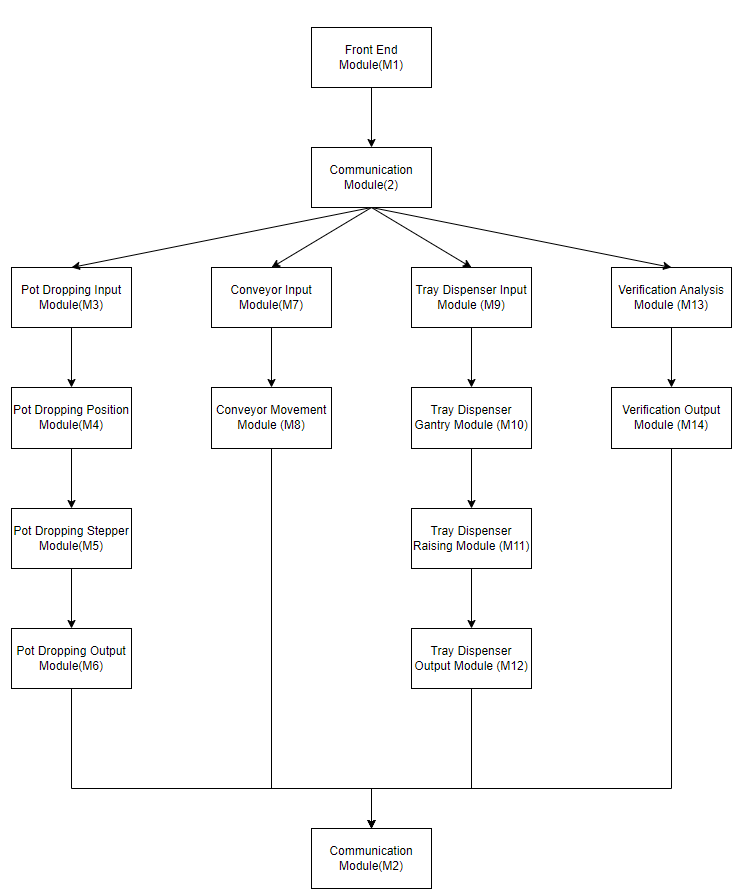
\includegraphics[width=0.9\textwidth]{ModuleGuide.png}
\caption{Use hierarchy among modules}
\label{FigUH}
\end{figure}

%\section*{References}

\bibliographystyle {plainnat}
\bibliography{../../../refs/References}

\newpage{}

\end{document}